\documentclass{chi2008}
\usepackage{myStyleHardLink}
\usepackage{times}
%\title{\Cacophony: Taming Mobile Data Flows}
%\title{\Cacophony: An architecture for computing in chaotic systems}
%\title{\Cacophony: A system for adding value to context observations}
%\title{\Cacophony: A system for adding intelligence to context observations}
%\title{\Cacophony: A wrapper for occasional context}
%\title{\Cacophony: A glue for seams}
\title{\Cacophony:\\ A System that Listens to the Internet of Things}
\numberofauthors{2} 
\author{
\alignauthor
Donald J. Patterson and Aaron Pecson\\
       \affaddr{Department of Informatics}\\
       \affaddr{University of California, Irvine, USA}\\
       \email{ \{djp3,apecson\}@uci.edu}
}


\begin{document}

\conferenceinfo{UbiComp'11,} {September 17--21, 2011, Beijing, China} 

\CopyrightYear{2011}

\crdata{TBD} 



\date{\today}
% Just remember to make sure that the TOTAL number of authors
% is the number that will appear on the first page PLUS the
% number that will appear in the \additionalauthors section.

\maketitle
\begin{abstract}

In this paper we describe a system for the intelligent management of data flows.
We describe our architecture and test it in real world situations.  We discuss
the use cases and failure cases for this technology.

\end{abstract}


\section{Introduction and Related Work}

Cacophony is a system that provides computational assistance with 
obtaining data from sources or sensors that are on the network, but not always
available or up to date.  It is particularly designed to address contextual data
sources and in particular supports sources of data that are human authored.

\donNote{I need to introduce enough of Cacophony to compare it to liquid, but I
also want a scenario quickly and want people to get their head around it
quickly}






\subsection{Scenario}

which may Where sensors is
interpretted broadly to include any source of information of context
information.

Cacoph

If you consider sensors as delivering samples of the real world over time and
then send those samples through a network, the samples can be conceptualized as
a flow.to 


The idea of using data flows as perspective from which to manage contextual data
is heavily influenced by work in streaming databases and introduced to the
UbiComp community through the liquid system developed by Heer
et.al.~\cite{HeerNBH03}.  Liquid was a broad conceptual approach to context
aware data delivery that was inspired by work in streaming databases.  The
primary goal of liquid was to create links between nodes which incrementally
gathered, processed and delivered information to interested parties.

Cacophony is similar in that it also provides an architecture for connecting
computation nodes that deliver data from a source through a series of
transformations and aggregations to a sink node.

The main architectural difference between liquid and Cacophony is that liquid
made the assumption that the underlying data was continuously available.
Cacophony in contrast assumes that the underlying data is hidden and only
occassionally is an observation made that provides information about the hidden
variable of interest.  Cacophony assumes that the observations are noisy and not
always available.

Liquid also focussed on data discovery and alerting mechanisms.  Both of these
aspects of data aggregation are important, but are secondary to Cacophony's goal
of revealing hidden, occasionaly observable data.  Data discovery and alerting
mechanisms are both services that can be built on top of Cacophony and are not
central to it's focus on aggregation and statistical interpretation. 

Liquid and cacophony both take the perspective that context information is
maintained in a distributed fashion across multiple physical and organizational
boundaries.

Liquid makes some claims about it's ability to reroute queries in order to
follow mobile entities.  Cacophony does not attempt to reroute its data flows
beyond the mechanisms supported by the underlying networking protocols.  Once a
source of data is provided to Cacophony, Cacophony assumes that the data is
available at that location for all time.

In contrast, cacophony does provide robust mechanisms for rapid duplication of
streams.  

Another way of looking at cacophony is not as a competitor to liquid, but as a
wrapper for liquid. 

If liquid performs distributed "queries", Cacophony performs distributed
statistically learning of context.  Liquid's primary focus is data discovery,
cacophony is about robust prediction of context.

Cacophony is not really an architecture for "streaming data" as much as
"streaming computation" which is presenting interpretations of instantaneous
data.

liquid encodes the idea of entities.  Cacophony supports entity prediction, but
doesn not expect a particular semantic on the underlying data.



Is there prior work before liquid?

What has come after liquid?  Does it relate?
\cite{Hong2004}


How do we handle privacy? We don't.  This is not about privacy it is about data
aggregation.  

\donNote{bad answer}


\subsection{Ideas}

The questions can be presented in a way that creates the least hassle for users
to answer i.e. Multiple Choice, Radio Button Ratings etc.

Their answers can be
stored and plotted on charts and graphs to give a flow of the general "time
based" information. 

For
example, a person wants get dinner at a restaurant, but doesn't want to be
bothered by long lines or noisy atmosphere. He can query Cacophony to find out
what the estimated wait time and atmosphere is like. 

Cacophony should also
present a percentage of accuracy based on the frequency of answered questions,
in a given time frame, for that location.


\section{Architecture}

We propose
to implement a reference version of the architecture shown in
figure~\ref{fig:architecture}.

\begin{figure}
\begin{center}
    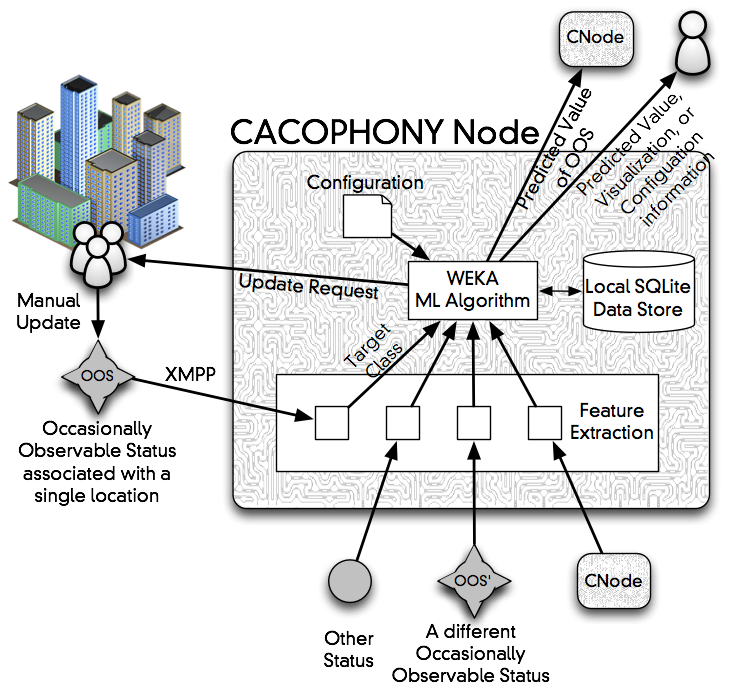
\includegraphics[width=\columnwidth, keepaspectratio=true]{images/architecture.png}
	\caption{\label{fig:architecture}left: Architecture of CACOPHONY, right: CNode Network}
\end{center}
\end{figure}


The basic organizing unit in CACOPHONY is the CACOPHONY Node (CNode).  A CNode
is always paired 1 to 1 with an occasionally observable status, $OOS$, that is associated with
a single location (shown on the left of figure~\ref{fig:architecture}).  It is
occasionally observable because it represents a random variable that is manually
updated by people.  When it is not observable it is a ``hidden" state in the
sense used in machine learning literature.  We also we mean that it is technically
occasionally observable to our CNode through the internet.  When our CNode would
like to know the current value of $OOS$ it is sometimes hidden because it has
not been manually updated recently and it is sometimes hidden because it is
inaccessible through the network.  Without loss of generality, but in keeping with the motivating example of
observing crowds, an example of such a variable might be the
number of people at a bus stop, the number of people in a train station lobby, or the
number of people in line at a movie theatre.

The value of $OOS$ is something that people would like continuous knowledge of.
This is represented in the figure by the icon in the upper right.  This user
could directly observe $OOS$, but because it is only occasionally observable, it
usually isn't up to date. So when users want to know the value of $OOS$, they
instead ask the associated CNode which provides a predicted value based on
a model that is learned by the CNode. 

Internally the CNode uses a machine learning (ML) algorithm to model and predict the
value of $OOS$.  We do not propose to develop new ML algorithms for this task,
instead we intend to incorporate the WEKA~\cite{Hall2009} ML algorithms into the
reference architecture.

$OOS$ is actually maintained on a status update site like Facebook.  On this
site there must be a page which represents the current crowd of people at a given
single location.  This requires creating a new site page for each location that
you wish to model and a paired CNode must be running somewhere to do the
modeling.  We intend to build our initial reference implementation to work with
Facebook and our initial CNode implementation to run in a Java virtual machine
located on a cloud computing service such as Amazon's EC2 service.  

The $OOS$
may be updated by anyone in the same way wiki pages are edited.  When this
happens the CNode will be immediately updated using a real-time update
standard.  Our reference implementation will initially use an XMPP notification
service called SuperFeedr.  This eliminates the need for polling by the CNode.
An alternative is PubSubHubbub which is supported by Google.

When the $OOS$ is updated the CNode is notified and immediately a collection of
features are polled to determine their current values.  This is represented by
the 3 icons on the bottom of the figure.  The figure only shows 3 sources, but
in general any number of sources are possible.  A variety of \emph{types} of sources
are also possible.  The format of the sources are only limited by the quantity
of feature extraction plug-ins that are available that are able to translate the
original feature into a data type that can be used by WEKA.  As these sources
may require some limited natural language understanding, our reference
implementation will used the OpenNLP
project\footnote{http://incubator.apache.org/opennlp/}.  The network location of
the $OOS$, the locations of the features and the feature extraction plug-ins to
use are all described in a configuration file that is part of the state of the
CNode.

When the CNode gets the current values of the feature vectors, it pairs them
with the recently pushed value of the $OOS$ and stores it locally in a
datastore.  This will be implemented as a SQLite database in our reference
implementation.  This datastore becomes the source of training data from which
the ML algorithm models the instantaneous statue of $OOS$. Whenever a new data
value is pushed over XMPP from $OOS$ the ML algorithm relearns a new model.

When a user (in the upper right) wishes to know the value of the $OOS$, the ML
algorithm has three different kinds of answers.  The first is to deliver the
most recently pushed $OOS$ value.  This may be stale or subject to spamming or
inaccuracy.  The second is to poll the \emph{features} for current values and then use
those in conjunction with a locally stored model to deliver a predicted value to
the user.  Provided the ML algorithm supports it and estimate of confidence can
be paired with the answer.  This is more robust to spoofing, but slower. A third method is for the CNode to poll friendly
observers that are in the vicinity of the $OOS$ and request that they update the
value of the $OOS$ on behalf of the requesting user. This is better in the face
of drastically unusual circumstances, but prone to human failure. Each of these types of
requests are appropriate for different needs based on accuracy, latency and privacy concerns.

Adding the ability to poll users to update the $OOS$ requires our system to tie
into a service like Google Latitude to locate observers.  While this is not a
key component of the CNode reference implementation, it will be a component of
the Phase II web portal. 

This architecture has several interesting implications. First, because the ML
algorithm is getting feature values whenever a new $OOS$ value is pushed over
XMPP, before it retrains itself, it can evaluate it's own accuracy by using the
new $OOS$ value as a testing example.  Statistics on historical accuracy can be
maintained locally for reference by users.  Secondly, internal state can be
requested as easily as predictions by outside users.  Because the systems state
is entirely encapsulated by the configuration file and the SQLite data base,
cloning the CNode, is as simple as coping those two items.   This enables the
rapid forking of successful CNodes for deployment at other locations or in
parallel situations which requires only small changes to the configuration file.
If historical data is not desired, the node can be cloned simply by requesting
it's configuration file.  Thirdly, external users may desire a prediction that
has more context than simply a value (and possibly a confidence).  It is simple
to deliver a graph of historical values, or predicted future values as a web
page or generated graphic file.  These can be embedded in web pages for more
user friendly monitoring of the $OOS$.

Lastly, CNodes can be thought of as representing semantic concepts and can be
chained together so that they predict and depend on each other.  For example,
predicting the number of
people in an entire mall could be based on predictions from the number of people in the food court,
and in the lines of each of the retail stores where each of those values are
themselves CNodes based on smaller observables.  Support for loop detection is
necessary, which can be managed by sending traces of data source flow graphs whenever
a configuration file is changed.  This will be necessary for data transparency
also.



\section{Discussion}
This is the discussion




\section{Conclusions}

This is the amazing conclusion.


%\end{document}  % This is where a 'short' article might terminate

%ACKNOWLEDGMENTS are optional
\section{Acknowledgments}
The authors wish to acknowledge the generous support of the U.S. National
Science Foundation through grant number HCC: 0713562.

\bibliographystyle{abbrv}
\bibliography{myBibCleanHardLink}
\balancecolumns
% That's all folks!
\end{document}
